% this file is called up by thesis.tex
% content in this file will be fed into the main document

\chapter{Fundamentals} % top level followed by section, subsection
This chapter explains the basic theory of 3D reconstruction and Structure from Motion. All information referred to herein can be found in \cite{HartleyMultipleView}. It also includes brief overview of sensor fusion made with the use of accelerometer, gyroscope and magnetometer data. 

% ----------------------- contents from here ------------------------
\section{3-D reconstruction in general}
There are many possibilities of performing reconstruction, starting from two-view reconstruction, multiple-view reconstruction and ending with the use of stereo calibrated cameras like the ones used in Kinect[reference]. Reconstruction can also be performed with a single hand-held camera either from a video or a sequence of images. As little as two pictures taken from different angles of a single object are sufficient to perform 3D model generation. Reconstruction process consists of the following steps:
\setlist[2]{noitemsep} % sets the itemsep and parsep for all level two lists to 0
\setenumerate{noitemsep} % sets no itemsep for enumerate lists only
\begin{enumerate}
\item \textbf{Image Acquistion}, where images are acquired 
\item \textbf{Feature extraction and corresponding points matching}, where distinctive features are extracted from the images and compared
\item \textbf{Fundamental \& Essential Matrices}, where matrices meeting the requirements of basic epipolar geometry are calculated
\item \textbf{Camera parameters estimation}, where external and internal camera parameters are estimated
\item \textbf{Triangulation}, where camera projection matrices are composed and used in order to calculate 3D cloud points
\end{enumerate}
\subsection{Feature extraction and corresponding points matching}
Usually, each image used in reconstruction has to be analysed in order for the dstinctive features to be found. Afterwards all features in images are compared in order to find corresponding matches(\ref{fig:correspondingMatches}).
\begin{figure}[p]
    \centering
    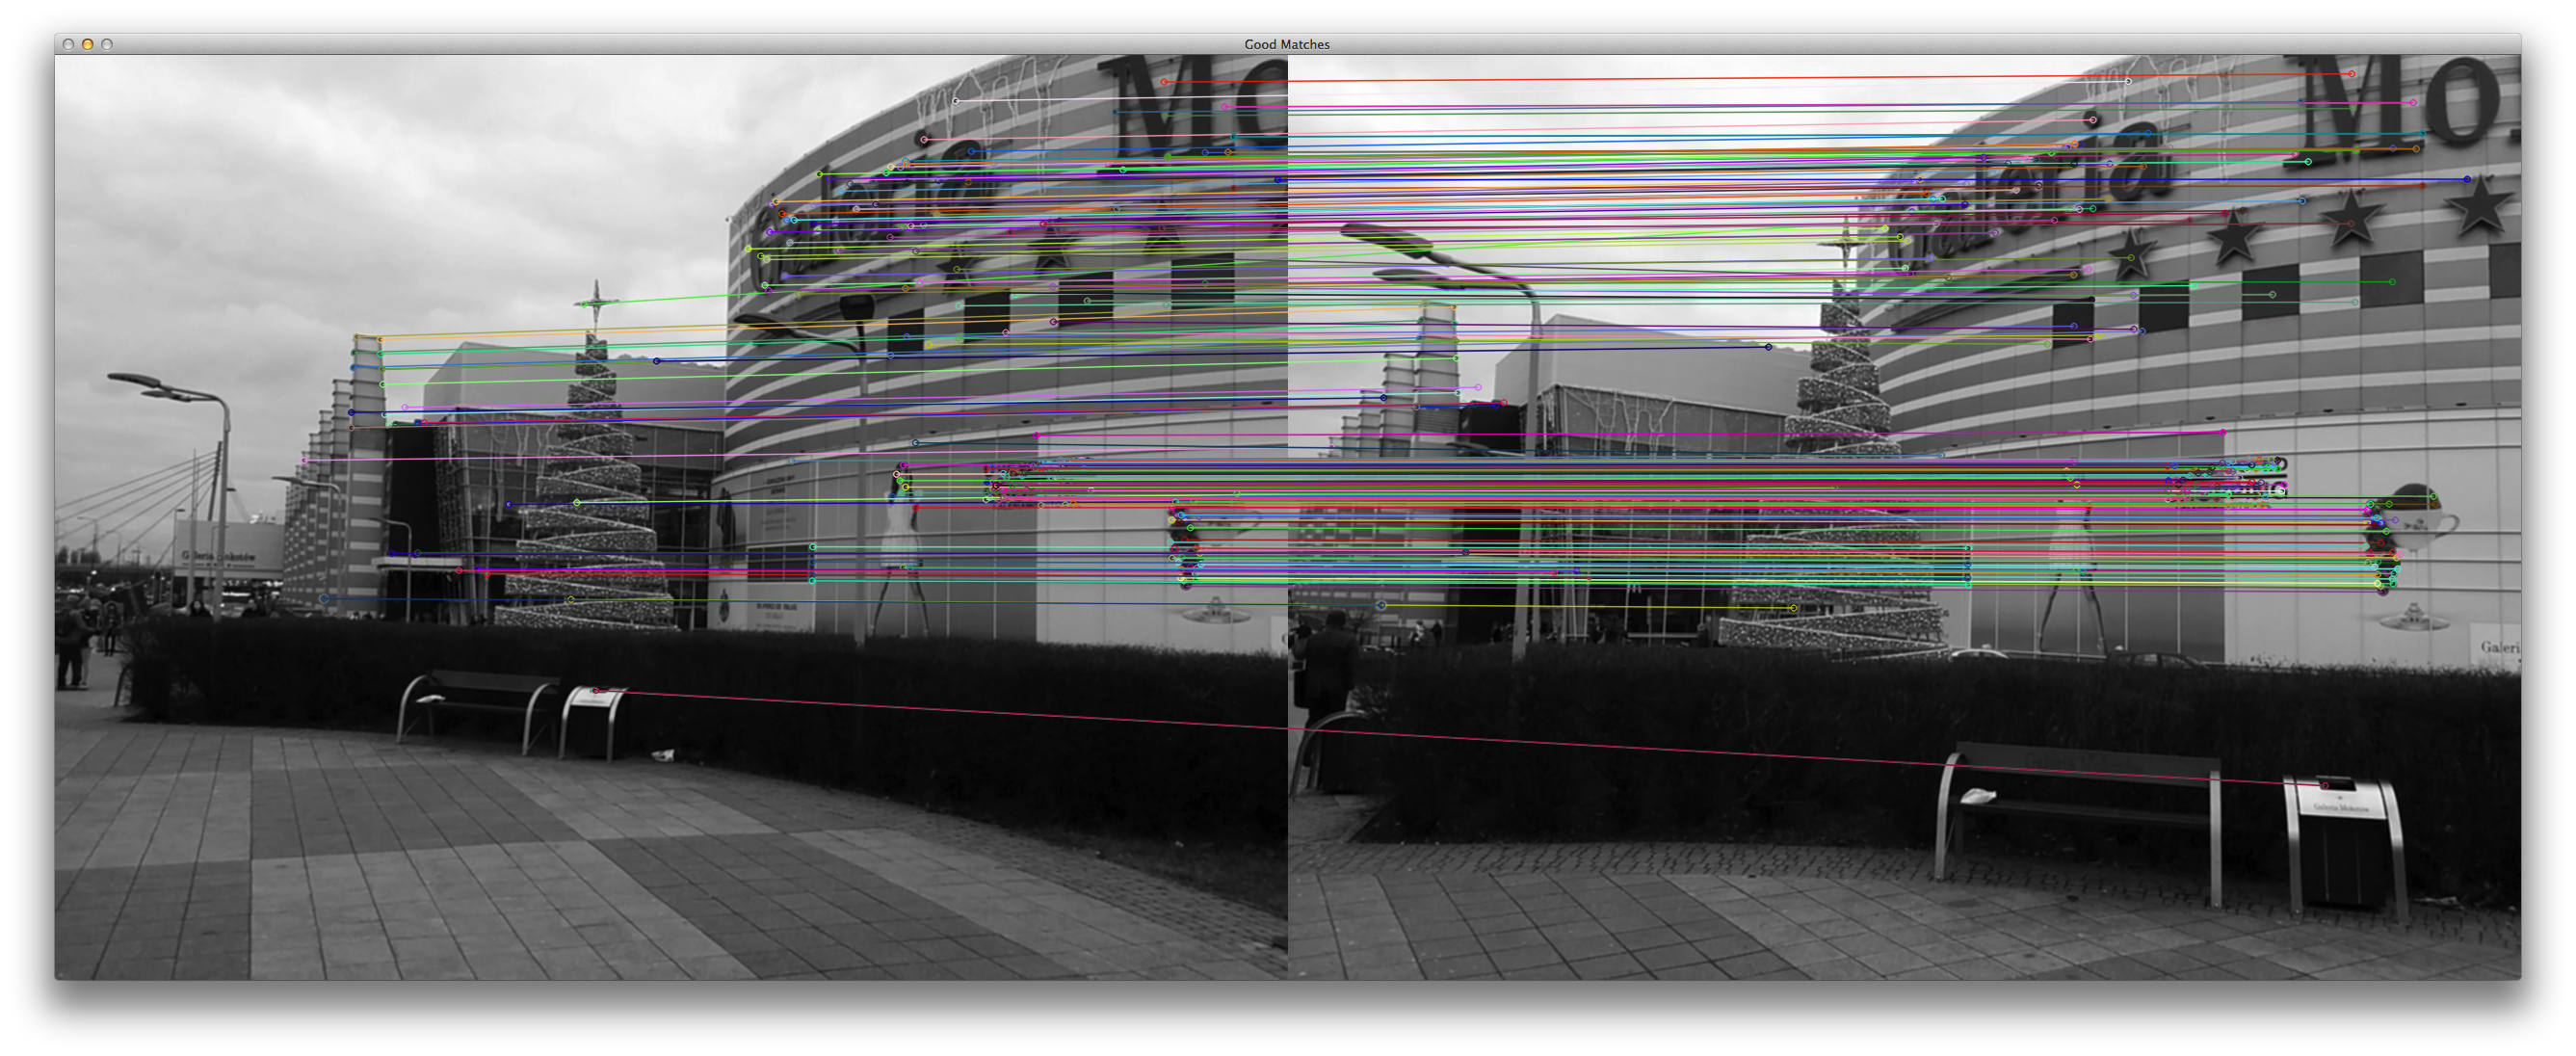
\includegraphics[width=0.8\textwidth]{correspondingMatching}
    \caption{}
    \label{fig:correspondingMatches}
\end{figure}
There are multiple features detectors and extractors available for use \url{$http://en.wikipedia.org/wiki/Feature_detection_%28computer_vision%29$}. Some of them are more suitable for edge detection, while others are best used for corner or blob detection. One of the most popluar and robust feature detection method is scale-invariant feature transform (SIFT) \url{http://en.wikipedia.org/wiki/Scale-invariant_feature_transform}. The use of these descriptors allows for detecting local features in images and describing them with metrics including scale, rotation and translation invariant.
\subsection{Fundamental \& Essential Matrix estimations}
Once proper matches are found, it can be proven that there exsists Fundamental matrix F for which the following equation is satisfied:
\begin{equation} \label{eq:fundamntalEquation}
{x}^{'T} * F * x = 0
\end{equation} 
where $x$ and ${x}_{'}$ are uncalibrated notions of points correspondence \cite{HartletMultipleView}TODO chapter. It is known that soultuions of this equation are highly sensitive to the occurence of outliers. Usually, to make fundamental matrix estimations more accurate some outliers removing algorithms need to be used. One of the most robust approaches includes the use of of RANdom SAmple Consensus (\gls{ransac}) \url{http://en.wikipedia.org/wiki/RANSAC}. The example of sample fitting can be seen in \ref{fig:RANSACFitting}
\begin{figure}[p]
    \centering
    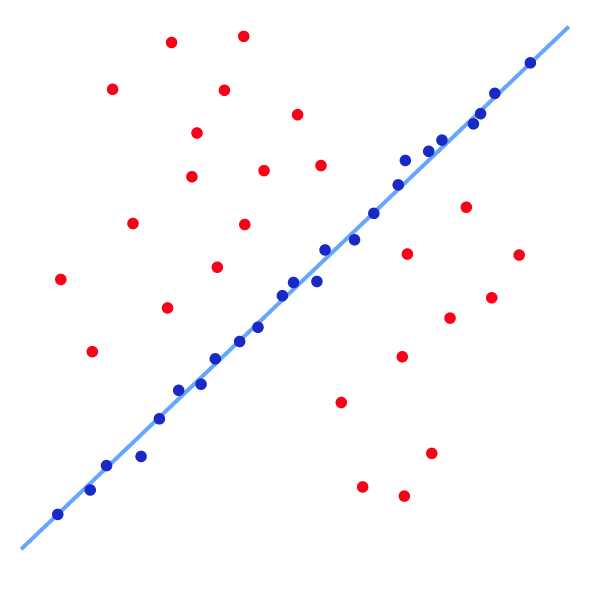
\includegraphics[width=0.8\textwidth]{RANSACFitting}
    \caption{RANSAC fitting for 2D image TODO reference}
    \label{fig:RANSACFitting}
\end{figure}
Its basic idea relies on choosing a random subset from among all matches, solving a problem of reduced dataset and establishing how many points from the original set satisfy the equation.
The use of F matrix allows for calculating epipolar lines for each point (\ref{fig:EpipolarGeometry}). These lines cross exactly the same points in both images and can be used for dense feature matching sinces matches need to be searched for exclusively in the surroundings of these lines.
\begin{figure}[p]
    \centering
    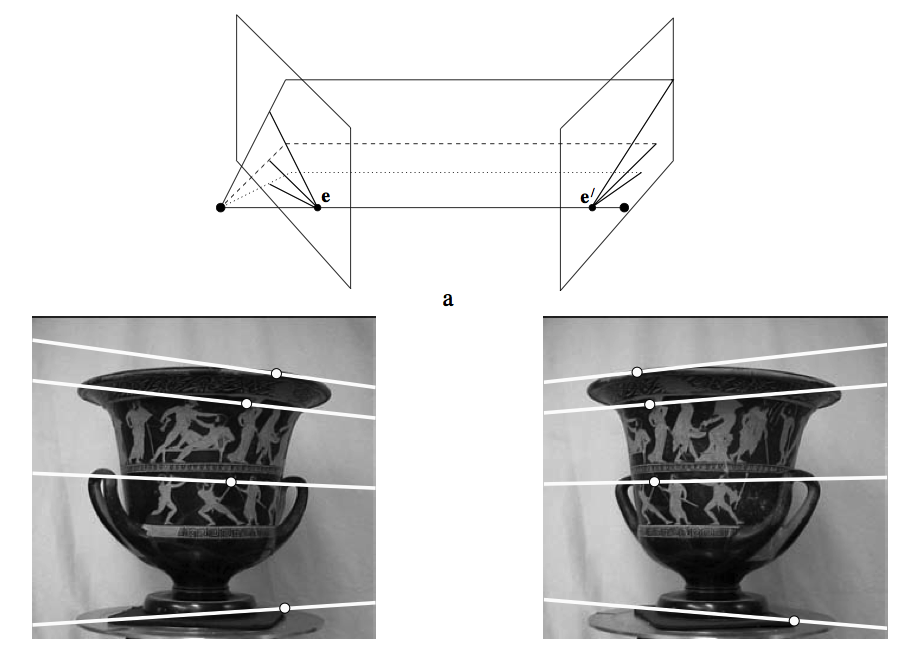
\includegraphics[width=0.8\textwidth]{EpipolarGeometry}
    \caption{Epipolar lines found in an image of a vase TODO reference}
    \label{fig:EpipolarGeometry}
\end{figure}
When enough inliers are found, points that do not satisfy the equation can be removed from further processing.
Once internal camera parameters K are known, the image points found can be calibrated and expressed in camera reference position system. Such calibrated points satisfy the following essential matrix E equation:
\begin{equation} \label{eq:essentialEquation}
{x}_{c}^{'T} * E * x_{c} = 0
\end{equation} 
which is very similar to fundamental equation \ref{eq:fundamntalEquation}. This results in:
\begin{equation} \label{eq:essentialFundamentalRelation}
E = K^{T} * F * K
\end{equation} 
with $K$ being the internal camera parameters. This equation \ref{eq:essentialFundamentalRelation} is important in terms of decomposition of F matrix to relative rotation and translation.
\subsection{Camera parameters estimations}
Internal camera parameters are expressed by the following matrix:
\begin{equation}
\begin{bmatrix}
\alpha _{x} &  & x_{0} \\ 
 & \alpha _{y} & y_{0}\\ 
 &  & 1
\end{bmatrix}
\end{equation}
where αx = fmx and αy = fmy represent the focal length of the camera expressed in pixel dimensions in the x and y direction respectively. 
Similarly, x ̃0 = (x0,y0) is the principal point of pixel dimensions. These parameters need to be calculated only once for each camera model. Cameras can be calibrated with special reference boards of the known dimensions and chracteristics.
For the proper 3D reconstruction it is essential to properly estimate external camera parameters, such as rotation (orientation angles of the camera) and global postition of the camera. It is often the case in 3D reconstruction that these parametrs are not known. However, it is showed in Chapter 9 of Multiple View Geometry in Computer Vision (\cite{HartleyMultipleView}), how essential matrix can be decomposed using Singular Value Decomposition \gls{svd} to relative camera positioning system of two projections:
\begin{equation}
 P1 = K * \begin{bmatrix}I\mid 0\end{bmatrix}
\end{equation}
the second one is equal to 
\begin{equation}
 P2 = K * \begin{bmatrix}RDiff\mid tDiff\end{bmatrix}
\end{equation}
Unfortunately, there are four possible solutions for such a decomposition and it is not always possible to identify the correct one.
\subsection{Points Triangulation}
Once internal and external (global or relative) camera parameters are calculated, the triangulation can be performed in order to acquire an up-to-affine reconstruction model (\ref{eq:3Dreconstruction}).
\begin{figure}[p]
    \centering
    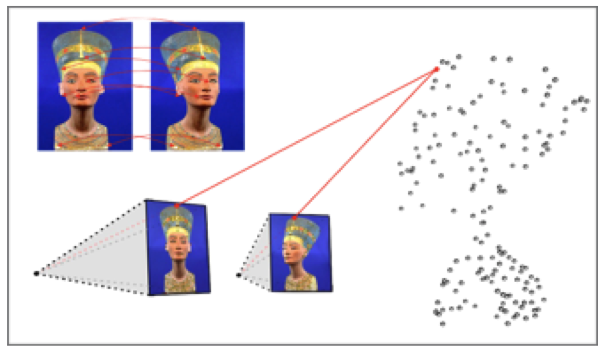
\includegraphics[width=0.8\textwidth]{3Dreconstruction}
    \caption{}
    \label{fig:3Dreconstruction}
\end{figure}
The only elemnt that cannot be determined in such a relative case is the scale. This process is described in detail in [TODO hartley chapter 10].
\section{Structure from Motion}
The term "Structure from Motion(SfM)" refers to the reconstruction performed from the consecutive sequences of a moving camera. It is a popular research topic and the two main approaches, namely the Pose Estimation and Homography Estimation, can be used for the [urposes of reconstructing a 3D model of an object.
\subsection{3D Pose Estimation}
Assuming that some of the 3D cloud points are already known, the matches between 2D features in a new image and 3D point cloud positions can be established. Such 3D-2D matches can be used to estimate the camera position. This allows for reconstructing new 3D points and merging them smoothly into a functional model. Unfortunately,  this process is also highly sensitive to the occurence of outliers, therefore adequate measeures have to be undertaken to reduce their influence. One of the main advanteges of this method is its speed. On the other hand, its effectiveness relies strongly on the exising 3D cloud quality. 
\subsection{Homography estimation}
A new image can be reconstructed with a previous one in a standard way in order to recive an up-to-scale 3D model. Afterwards, a newly acquired model can be merged into existing one using homography estimation between the coresponding 3D points. Such a strategy is slower than the previous one, but it is not influenced by the quality of the existing 3D model. Although it is highly sensitive to outliers as well, if used properly it can produce more new 3D points.
\subsection{Structure Adjustment}
Special refinement methods can be used to compensate for an error of mismatched points propagating through images. They include. among others, Bundle Adjustment\gls{ba} \url{http://en.wikipedia.org/wiki/Bundle_adjustment}. The algorithm, using the information concerning the corresponding matches between multiple sets of images, iteratively modifies either both the camera external paramaters and 3D points positions or one of them. The main disadvantage of the method is its execution time. It is too time-consuming to use it in real-time applications. The basic idea of BA is expresed in figure \ref{fig:BundleAdjustment}.
\begin{figure}[p]
    \centering
    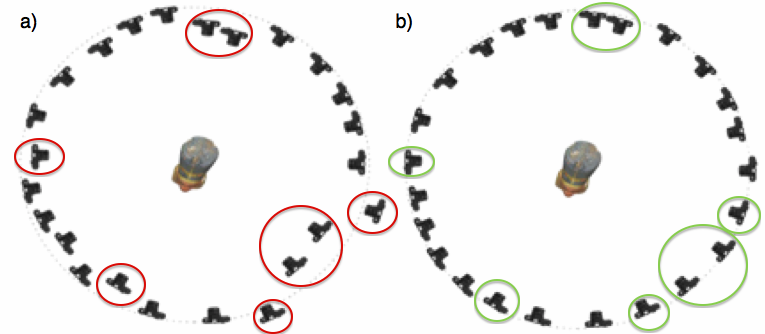
\includegraphics[width=0.8\textwidth]{BundleAdjustment}
    \caption{TODO reference}
    \label{fig:BundleAdjustment}
\end{figure}
\section{Mobile Sensors overview}
There are many sensors available in the nowadays smartphones, such as accelerometer, gyroscope, magnetometer, barometer, GPS, etc. All of them have their advantages and disadvanteges, and thus the errors of some might be compensated for with the strengths of the others in otrder to, for example, accuretely compute camera rotation angles.
\subsection{Accelerometer}
An accelerometer is a device that measures acceleration along 3 axes of the device [reference]. Generally, an accelerometer allows for measuring total acceleration by sensing what force is applied to its micro strings. An accelerometer, which lies on a flat surface perpendicular to the Earth's surface will indicate approximately 1G upwards. This gravitation vector can be used to caculate the relative camera rotation, but it is difficult to define to which direction the gravity vector points when the device is moving in not a linear manner. The gravity vector is obtained from the accelerometer data and tracked during unexpected movements with the used of gyroscope sensor.
\subsection{Gyroscope}
A gyroscope is a device for measuring or maintaining orientation, based on the principles of conservation of angular momentum [reference]. A standard gyroscope consists of a spinning wheel mounted on two gimbal rings, which allows it to rotate in all three axes. The spinning wheel will resist changes in orientation, due to an effect of the conservation of angular momentum. A conventional gyroscope measures orientation, in contrast to MEMS (Micro Electro-Mechanical System) types, which measure
angular rate, and are therefore called rate-gyros [reference]. MEMS gyroscopes contain vibrating elements to measure the Coriolis effect. In the end the angular velocity can be calculated in each axis. It is important to note that whereas the accelerometer and the magnetometer measure acceleration and angle relative to the Earth, gyroscope measures angular velocity
relative to the body.
\subsection{Magnetometer}
A magnetometer is an instrument used to measure the strength and/or direction of the magnetic field in the surrounding area of the instrument. Its main idea works in the same manner as the conventional compass'. With some magentometers magnetic field can be meeasured in 3 directions, relative to the spatial orientation of the device [reference]. Using magnetometers allows for estimating relative position in geomagnetic north position system. 
\subsection{Sensor Fusion}
Sensor fusion is the process of combining sensory data derived from disparate
sources in a way that the resulting information is to some extent more valuable than it would be possible should these sources be used individually. The term "more valuble" in this case may mean "more
accurate", "more complete", or "more dependable", or refer to the result of an emerging view, such
as stereoscopic vision (calculation of depth information by combining two-dimensional
images from two cameras at slightly different viewpoints) [reference]. One of the strategies available is Kalman filtering(\ref{fig:Kalmann})
\begin{figure}[p]
    \centering
    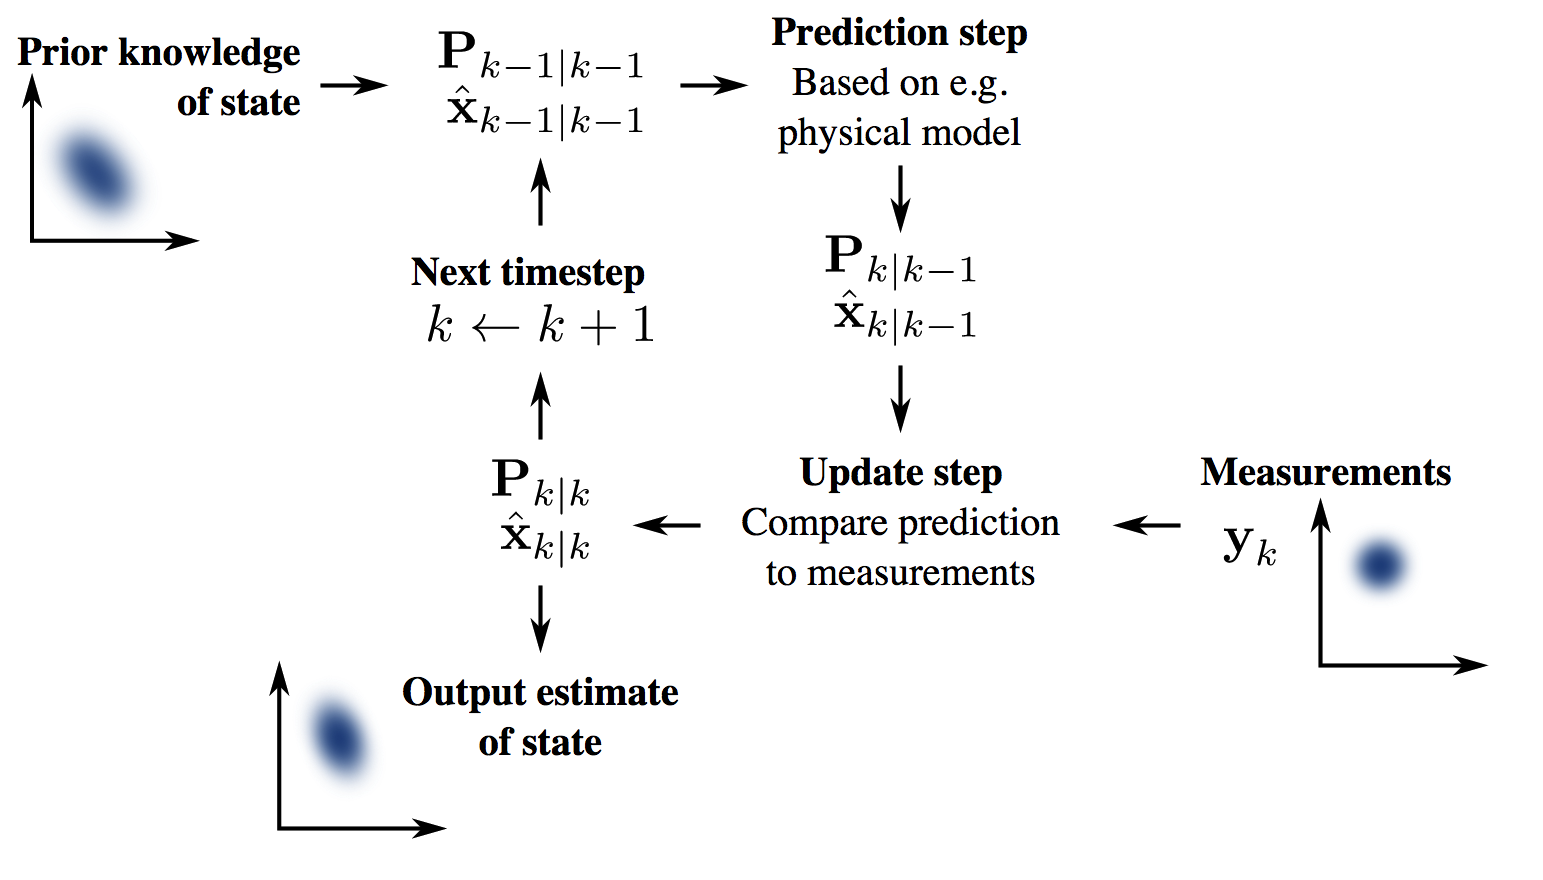
\includegraphics[width=0.8\textwidth]{Kalmann}
    \caption{}
    \label{fig:Kalmann}
\end{figure}
This approach is used in Sesnor Fusion available in Android API, where the gravity vector calculateion is enhanced with the accelerometer and gyroscope data. The gravity vector can be decomposed in order to estimate the camera's rotation angles. Magnetometer can be used optionally in order to acquire rotation angles referrenced to the Earth's coordinate system. However, magnetometer is sensitive to changes in the electromagnetic fields, therefore its measurement can be noisy in confined spaces filled with electronic devices. Substracting gravity from the actual acceleration measurements allows for estimating linear acceleration. The use of linear acceleration makes it possible to measure the relative change of the device's translation. However, it requires a double integration over time, which results in increasing the translation's noise. It is important to note that calculating rotation is significantly more accurate than estimating the translation. 


% ---------------------------------------------------------------------------
% ----------------------- end of thesis sub-document ------------------------
% ---------------------------------------------------------------------------
